\documentclass{standalone}
\usepackage{tikz}
\usetikzlibrary{patterns, positioning}

\begin{document}
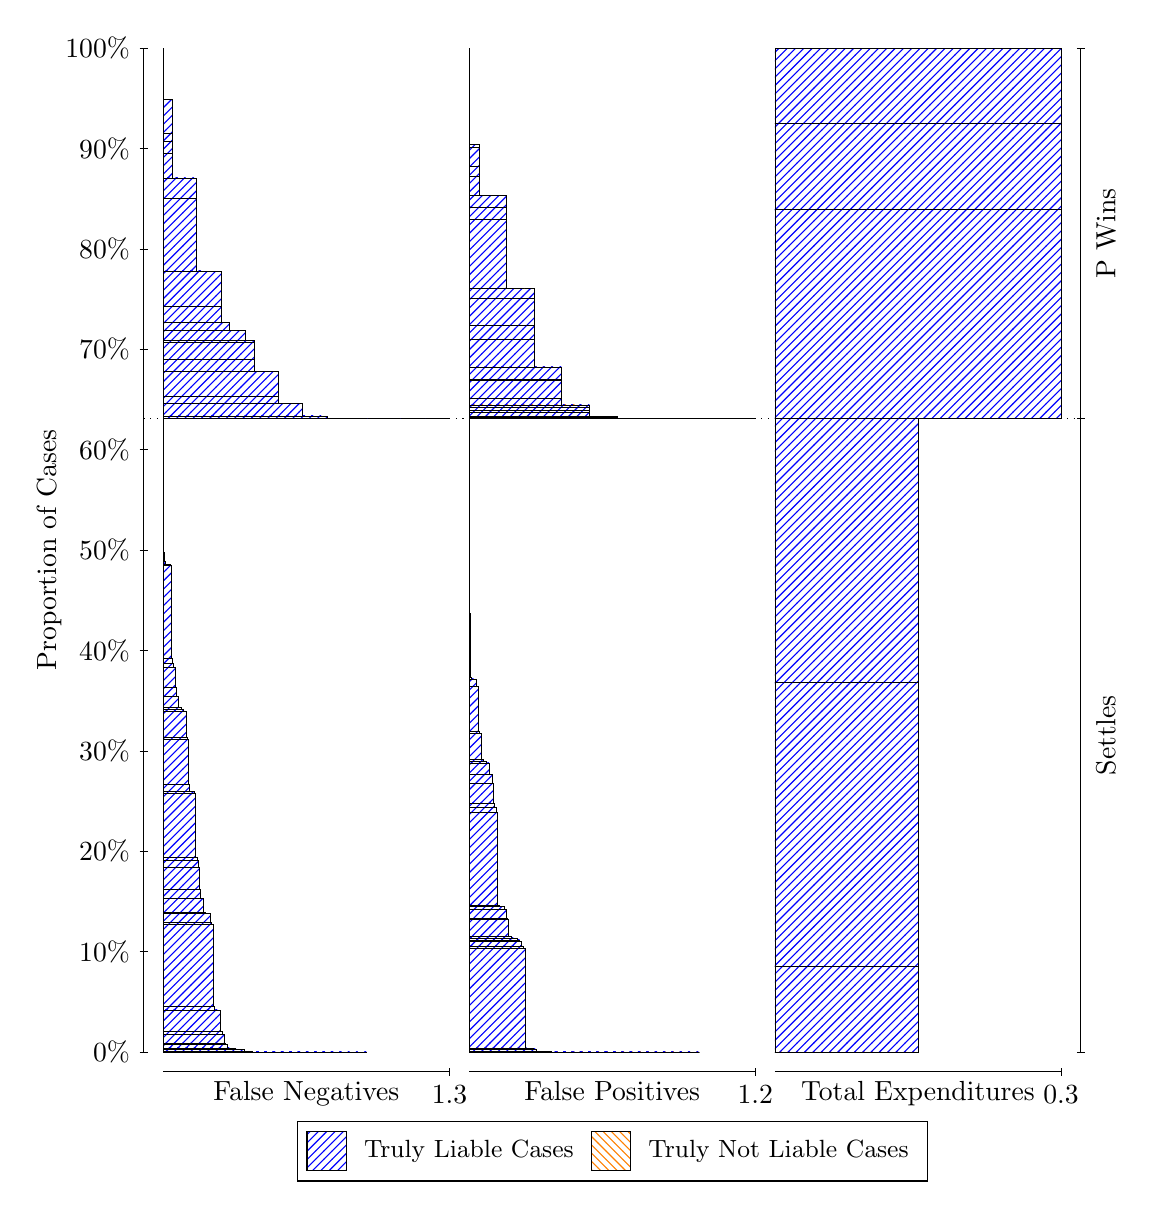
\begin{tikzpicture}
\draw[black, very thin] (1.5,1.75) -- (1.5,14.5);
\node[rotate=90, anchor=center] at (0.3, 8.125) {Proportion of Cases};
\draw[black, very thin] (1.45,1.75) -- (1.55,1.75);
\node[anchor=east] at (1.45, 1.75) {0\%};
\draw[black, very thin] (1.45,3.025) -- (1.55,3.025);
\node[anchor=east] at (1.45, 3.025) {10\%};
\draw[black, very thin] (1.45,4.3) -- (1.55,4.3);
\node[anchor=east] at (1.45, 4.3) {20\%};
\draw[black, very thin] (1.45,5.575) -- (1.55,5.575);
\node[anchor=east] at (1.45, 5.575) {30\%};
\draw[black, very thin] (1.45,6.85) -- (1.55,6.85);
\node[anchor=east] at (1.45, 6.85) {40\%};
\draw[black, very thin] (1.45,8.125) -- (1.55,8.125);
\node[anchor=east] at (1.45, 8.125) {50\%};
\draw[black, very thin] (1.45,9.4) -- (1.55,9.4);
\node[anchor=east] at (1.45, 9.4) {60\%};
\draw[black, very thin] (1.45,10.675) -- (1.55,10.675);
\node[anchor=east] at (1.45, 10.675) {70\%};
\draw[black, very thin] (1.45,11.95) -- (1.55,11.95);
\node[anchor=east] at (1.45, 11.95) {80\%};
\draw[black, very thin] (1.45,13.225) -- (1.55,13.225);
\node[anchor=east] at (1.45, 13.225) {90\%};
\draw[black, very thin] (1.45,14.5) -- (1.55,14.5);
\node[anchor=east] at (1.45, 14.5) {100\%};

\draw[black, very thin] (13.4,1.75) -- (13.4,14.5);
\draw[black, very thin] (13.35,1.75) -- (13.45,1.75);
\node[anchor=west] at (13.35, 1.75) {};
\draw[black, very thin] (13.35,9.7946) -- (13.45,9.7946);
\node[anchor=west] at (13.35, 9.7946) {};
\draw[black, very thin] (13.35,14.5) -- (13.45,14.5);
\node[anchor=west] at (13.35, 14.5) {};

\draw[black, very thin, pattern color=blue, pattern=north east lines] (1.75,1.75) rectangle (4.3353,1.75);
\draw[black, very thin, pattern color=blue, pattern=north east lines] (1.75,1.75) rectangle (4.0558,1.75);
\draw[black, very thin, pattern color=blue, pattern=north east lines] (1.75,1.75) rectangle (4.0247,1.75);
\draw[black, very thin, pattern color=blue, pattern=north east lines] (1.75,1.75) rectangle (3.916,1.75);
\draw[black, very thin, pattern color=blue, pattern=north east lines] (1.75,1.75) rectangle (3.7763,1.75);
\draw[black, very thin, pattern color=blue, pattern=north east lines] (1.75,1.75) rectangle (3.7452,1.75);
\draw[black, very thin, pattern color=blue, pattern=north east lines] (1.75,1.75) rectangle (3.7142,1.75);
\draw[black, very thin, pattern color=blue, pattern=north east lines] (1.75,1.75) rectangle (3.6365,1.75);
\draw[black, very thin, pattern color=blue, pattern=north east lines] (1.75,1.75) rectangle (3.6055,1.75);
\draw[black, very thin, pattern color=blue, pattern=north east lines] (1.75,1.75) rectangle (3.4968,1.75);
\draw[black, very thin, pattern color=blue, pattern=north east lines] (1.75,1.75) rectangle (3.4657,1.75);
\draw[black, very thin, pattern color=blue, pattern=north east lines] (1.75,1.75) rectangle (3.4347,1.75);
\draw[black, very thin, pattern color=blue, pattern=north east lines] (1.75,1.75) rectangle (3.4036,1.75);
\draw[black, very thin, pattern color=blue, pattern=north east lines] (1.75,1.75) rectangle (3.3571,1.75);
\draw[black, very thin, pattern color=blue, pattern=north east lines] (1.75,1.75) rectangle (3.326,1.75);
\draw[black, very thin, pattern color=blue, pattern=north east lines] (1.75,1.75) rectangle (3.2949,1.75);
\draw[black, very thin, pattern color=blue, pattern=north east lines] (1.75,1.75) rectangle (3.2173,1.75);
\draw[black, very thin, pattern color=blue, pattern=north east lines] (1.75,1.75) rectangle (3.1863,1.75);
\draw[black, very thin, pattern color=blue, pattern=north east lines] (1.75,1.75) rectangle (3.1552,1.75);
\draw[black, very thin, pattern color=blue, pattern=north east lines] (1.75,1.75) rectangle (3.1241,1.75);
\draw[black, very thin, pattern color=blue, pattern=north east lines] (1.75,1.75) rectangle (3.0931,1.7506);
\draw[black, very thin, pattern color=blue, pattern=north east lines] (1.75,1.7506) rectangle (3.0776,1.7506);
\draw[black, very thin, pattern color=blue, pattern=north east lines] (1.75,1.7506) rectangle (3.0465,1.7506);
\draw[black, very thin, pattern color=blue, pattern=north east lines] (1.75,1.7506) rectangle (3.0155,1.7506);
\draw[black, very thin, pattern color=blue, pattern=north east lines] (1.75,1.7506) rectangle (2.9844,1.7508);
\draw[black, very thin, pattern color=blue, pattern=north east lines] (1.75,1.7508) rectangle (2.9378,1.7508);
\draw[black, very thin, pattern color=blue, pattern=north east lines] (1.75,1.7508) rectangle (2.9068,1.7508);
\draw[black, very thin, pattern color=blue, pattern=north east lines] (1.75,1.7508) rectangle (2.8757,1.7528);
\draw[black, very thin, pattern color=blue, pattern=north east lines] (1.75,1.7528) rectangle (2.8447,1.7533);
\draw[black, very thin, pattern color=blue, pattern=north east lines] (1.75,1.7533) rectangle (2.8136,1.7552);
\draw[black, very thin, pattern color=blue, pattern=north east lines] (1.75,1.7552) rectangle (2.7981,1.7552);
\draw[black, very thin, pattern color=blue, pattern=north east lines] (1.75,1.7552) rectangle (2.7825,1.7815);
\draw[black, very thin, pattern color=blue, pattern=north east lines] (1.75,1.7815) rectangle (2.767,1.7816);
\draw[black, very thin, pattern color=blue, pattern=north east lines] (1.75,1.7816) rectangle (2.736,1.7816);
\draw[black, very thin, pattern color=blue, pattern=north east lines] (1.75,1.7816) rectangle (2.7049,1.7859);
\draw[black, very thin, pattern color=blue, pattern=north east lines] (1.75,1.7859) rectangle (2.6739,1.7905);
\draw[black, very thin, pattern color=blue, pattern=north east lines] (1.75,1.7905) rectangle (2.6583,1.8016);
\draw[black, very thin, pattern color=blue, pattern=north east lines] (1.75,1.8016) rectangle (2.6273,1.8019);
\draw[black, very thin, pattern color=blue, pattern=north east lines] (1.75,1.8019) rectangle (2.5962,1.8023);
\draw[black, very thin, pattern color=blue, pattern=north east lines] (1.75,1.8023) rectangle (2.5652,1.8453);
\draw[black, very thin, pattern color=blue, pattern=north east lines] (1.75,1.8453) rectangle (2.5341,1.864);
\draw[black, very thin, pattern color=blue, pattern=north east lines] (1.75,1.864) rectangle (2.5186,1.9749);
\draw[black, very thin, pattern color=blue, pattern=north east lines] (1.75,1.9749) rectangle (2.5031,2.0076);
\draw[black, very thin, pattern color=blue, pattern=north east lines] (1.75,2.0076) rectangle (2.4875,2.0095);
\draw[black, very thin, pattern color=blue, pattern=north east lines] (1.75,2.0095) rectangle (2.472,2.2813);
\draw[black, very thin, pattern color=blue, pattern=north east lines] (1.75,2.2813) rectangle (2.4565,2.2844);
\draw[black, very thin, pattern color=blue, pattern=north east lines] (1.75,2.2844) rectangle (2.4254,2.2849);
\draw[black, very thin, pattern color=blue, pattern=north east lines] (1.75,2.2849) rectangle (2.3944,2.3301);
\draw[black, very thin, pattern color=blue, pattern=north east lines] (1.75,2.3301) rectangle (2.3788,3.3707);
\draw[black, very thin, pattern color=blue, pattern=north east lines] (1.75,3.3707) rectangle (2.3633,3.3955);
\draw[black, very thin, pattern color=blue, pattern=north east lines] (1.75,3.3955) rectangle (2.3478,3.5077);
\draw[black, very thin, pattern color=blue, pattern=north east lines] (1.75,3.5077) rectangle (2.3167,3.5131);
\draw[black, very thin, pattern color=blue, pattern=north east lines] (1.75,3.5131) rectangle (2.2857,3.5203);
\draw[black, very thin, pattern color=blue, pattern=north east lines] (1.75,3.5203) rectangle (2.2546,3.6998);
\draw[black, very thin, pattern color=blue, pattern=north east lines] (1.75,3.6998) rectangle (2.2236,3.8178);
\draw[black, very thin, pattern color=blue, pattern=north east lines] (1.75,3.8178) rectangle (2.208,4.0948);
\draw[black, very thin, pattern color=blue, pattern=north east lines] (1.75,4.0948) rectangle (2.1925,4.1899);
\draw[black, very thin, pattern color=blue, pattern=north east lines] (1.75,4.1899) rectangle (2.177,4.2171);
\draw[black, very thin, pattern color=blue, pattern=north east lines] (1.75,4.2171) rectangle (2.1615,5.0371);
\draw[black, very thin, pattern color=blue, pattern=north east lines] (1.75,5.0371) rectangle (2.1459,5.0563);
\draw[black, very thin, pattern color=blue, pattern=north east lines] (1.75,5.0563) rectangle (2.1149,5.0598);
\draw[black, very thin, pattern color=blue, pattern=north east lines] (1.75,5.0598) rectangle (2.0838,5.1505);
\draw[black, very thin, pattern color=blue, pattern=north east lines] (1.75,5.1505) rectangle (2.0683,5.7218);
\draw[black, very thin, pattern color=blue, pattern=north east lines] (1.75,5.7218) rectangle (2.0528,5.7475);
\draw[black, very thin, pattern color=blue, pattern=north east lines] (1.75,5.7475) rectangle (2.0373,6.0806);
\draw[black, very thin, pattern color=blue, pattern=north east lines] (1.75,6.0806) rectangle (2.0062,6.1051);
\draw[black, very thin, pattern color=blue, pattern=north east lines] (1.75,6.1051) rectangle (1.9751,6.1232);
\draw[black, very thin, pattern color=blue, pattern=north east lines] (1.75,6.1232) rectangle (1.9441,6.266);
\draw[black, very thin, pattern color=blue, pattern=north east lines] (1.75,6.266) rectangle (1.913,6.3841);
\draw[black, very thin, pattern color=blue, pattern=north east lines] (1.75,6.3841) rectangle (1.8975,6.6301);
\draw[black, very thin, pattern color=blue, pattern=north east lines] (1.75,6.6301) rectangle (1.882,6.6837);
\draw[black, very thin, pattern color=blue, pattern=north east lines] (1.75,6.6837) rectangle (1.8665,6.7513);
\draw[black, very thin, pattern color=blue, pattern=north east lines] (1.75,6.7513) rectangle (1.8509,7.9271);
\draw[black, very thin, pattern color=blue, pattern=north east lines] (1.75,7.9271) rectangle (1.8354,7.9463);
\draw[black, very thin, pattern color=blue, pattern=north east lines] (1.75,7.9463) rectangle (1.8043,7.9497);
\draw[black, very thin, pattern color=blue, pattern=north east lines] (1.75,7.9497) rectangle (1.7733,7.9821);
\draw[black, very thin, pattern color=blue, pattern=north east lines] (1.75,7.9821) rectangle (1.7578,8.1001);
\draw[black, very thin, pattern color=orange, pattern=north west lines] (1.75,8.1001) rectangle (1.75,8.1001);
\draw[black, very thin, pattern color=blue, pattern=north east lines] (1.75,8.1001) rectangle (1.75,9.7946);
\draw[black, very thin, pattern color=blue, pattern=north east lines] (1.75,9.7946) rectangle (5.3833,9.7946);
\draw[black, very thin, pattern color=blue, pattern=north east lines] (1.75,9.7946) rectangle (5.0728,9.7946);
\draw[black, very thin, pattern color=blue, pattern=north east lines] (1.75,9.7946) rectangle (4.7623,9.7946);
\draw[black, very thin, pattern color=blue, pattern=north east lines] (1.75,9.7946) rectangle (4.4517,9.7947);
\draw[black, very thin, pattern color=blue, pattern=north east lines] (1.75,9.7947) rectangle (4.4517,9.7948);
\draw[black, very thin, pattern color=blue, pattern=north east lines] (1.75,9.7948) rectangle (4.343,9.7948);
\draw[black, very thin, pattern color=blue, pattern=north east lines] (1.75,9.7948) rectangle (4.1412,9.7969);
\draw[black, very thin, pattern color=blue, pattern=north east lines] (1.75,9.7969) rectangle (4.1412,9.7983);
\draw[black, very thin, pattern color=blue, pattern=north east lines] (1.75,9.7983) rectangle (4.0325,9.7983);
\draw[black, very thin, pattern color=blue, pattern=north east lines] (1.75,9.7983) rectangle (3.8306,9.8293);
\draw[black, very thin, pattern color=blue, pattern=north east lines] (1.75,9.8293) rectangle (3.7219,9.8293);
\draw[black, very thin, pattern color=blue, pattern=north east lines] (1.75,9.8293) rectangle (3.7219,9.8293);
\draw[black, very thin, pattern color=blue, pattern=north east lines] (1.75,9.8293) rectangle (3.5201,9.9884);
\draw[black, very thin, pattern color=blue, pattern=north east lines] (1.75,9.9884) rectangle (3.4114,9.9886);
\draw[black, very thin, pattern color=blue, pattern=north east lines] (1.75,9.9886) rectangle (3.2095,10.08);
\draw[black, very thin, pattern color=blue, pattern=north east lines] (1.75,10.08) rectangle (3.2095,10.389);
\draw[black, very thin, pattern color=blue, pattern=north east lines] (1.75,10.389) rectangle (3.1009,10.393);
\draw[black, very thin, pattern color=blue, pattern=north east lines] (1.75,10.393) rectangle (3.1009,10.397);
\draw[black, very thin, pattern color=blue, pattern=north east lines] (1.75,10.397) rectangle (2.899,10.542);
\draw[black, very thin, pattern color=blue, pattern=north east lines] (1.75,10.542) rectangle (2.899,10.765);
\draw[black, very thin, pattern color=blue, pattern=north east lines] (1.75,10.765) rectangle (2.899,10.783);
\draw[black, very thin, pattern color=blue, pattern=north east lines] (1.75,10.783) rectangle (2.7903,10.914);
\draw[black, very thin, pattern color=blue, pattern=north east lines] (1.75,10.914) rectangle (2.5885,11.015);
\draw[black, very thin, pattern color=blue, pattern=north east lines] (1.75,11.015) rectangle (2.4798,11.218);
\draw[black, very thin, pattern color=blue, pattern=north east lines] (1.75,11.218) rectangle (2.4798,11.662);
\draw[black, very thin, pattern color=blue, pattern=north east lines] (1.75,11.662) rectangle (2.2779,11.662);
\draw[black, very thin, pattern color=blue, pattern=north east lines] (1.75,11.662) rectangle (2.2779,11.669);
\draw[black, very thin, pattern color=blue, pattern=north east lines] (1.75,11.669) rectangle (2.2779,11.669);
\draw[black, very thin, pattern color=blue, pattern=north east lines] (1.75,11.669) rectangle (2.1692,12.589);
\draw[black, very thin, pattern color=blue, pattern=north east lines] (1.75,12.589) rectangle (2.1692,12.851);
\draw[black, very thin, pattern color=blue, pattern=north east lines] (1.75,12.851) rectangle (1.9674,12.851);
\draw[black, very thin, pattern color=blue, pattern=north east lines] (1.75,12.851) rectangle (1.9674,12.851);
\draw[black, very thin, pattern color=blue, pattern=north east lines] (1.75,12.851) rectangle (1.8587,13.161);
\draw[black, very thin, pattern color=blue, pattern=north east lines] (1.75,13.161) rectangle (1.8587,13.311);
\draw[black, very thin, pattern color=blue, pattern=north east lines] (1.75,13.311) rectangle (1.8587,13.416);
\draw[black, very thin, pattern color=blue, pattern=north east lines] (1.75,13.416) rectangle (1.8587,13.844);
\draw[black, very thin, pattern color=orange, pattern=north west lines] (1.75,13.844) rectangle (1.75,13.844);
\draw[black, very thin, pattern color=blue, pattern=north east lines] (1.75,13.844) rectangle (1.75,14.5);
\draw[black, very thin, pattern color=orange, pattern=north west lines] (5.6333,1.75) rectangle (8.5558,1.75);
\draw[black, very thin, pattern color=blue, pattern=north east lines] (5.6333,1.75) rectangle (8.5558,1.75);
\draw[black, very thin, pattern color=orange, pattern=north west lines] (5.6333,1.75) rectangle (8.3978,1.75);
\draw[black, very thin, pattern color=blue, pattern=north east lines] (5.6333,1.75) rectangle (8.3978,1.75);
\draw[black, very thin, pattern color=orange, pattern=north west lines] (5.6333,1.75) rectangle (8.2399,1.75);
\draw[black, very thin, pattern color=blue, pattern=north east lines] (5.6333,1.75) rectangle (8.2399,1.75);
\draw[black, very thin, pattern color=blue, pattern=north east lines] (5.6333,1.75) rectangle (8.2048,1.75);
\draw[black, very thin, pattern color=orange, pattern=north west lines] (5.6333,1.75) rectangle (8.0819,1.75);
\draw[black, very thin, pattern color=blue, pattern=north east lines] (5.6333,1.75) rectangle (8.0819,1.75);
\draw[black, very thin, pattern color=blue, pattern=north east lines] (5.6333,1.75) rectangle (8.0468,1.75);
\draw[black, very thin, pattern color=orange, pattern=north west lines] (5.6333,1.75) rectangle (7.9239,1.75);
\draw[black, very thin, pattern color=blue, pattern=north east lines] (5.6333,1.75) rectangle (7.9239,1.75);
\draw[black, very thin, pattern color=blue, pattern=north east lines] (5.6333,1.75) rectangle (7.8888,1.75);
\draw[black, very thin, pattern color=blue, pattern=north east lines] (5.6333,1.75) rectangle (7.8537,1.75);
\draw[black, very thin, pattern color=orange, pattern=north west lines] (5.6333,1.75) rectangle (7.7659,1.75);
\draw[black, very thin, pattern color=blue, pattern=north east lines] (5.6333,1.75) rectangle (7.7659,1.75);
\draw[black, very thin, pattern color=blue, pattern=north east lines] (5.6333,1.75) rectangle (7.7308,1.75);
\draw[black, very thin, pattern color=blue, pattern=north east lines] (5.6333,1.75) rectangle (7.6957,1.75);
\draw[black, very thin, pattern color=orange, pattern=north west lines] (5.6333,1.75) rectangle (7.608,1.75);
\draw[black, very thin, pattern color=blue, pattern=north east lines] (5.6333,1.75) rectangle (7.608,1.75);
\draw[black, very thin, pattern color=blue, pattern=north east lines] (5.6333,1.75) rectangle (7.5729,1.75);
\draw[black, very thin, pattern color=blue, pattern=north east lines] (5.6333,1.75) rectangle (7.5378,1.75);
\draw[black, very thin, pattern color=blue, pattern=north east lines] (5.6333,1.75) rectangle (7.5027,1.75);
\draw[black, very thin, pattern color=orange, pattern=north west lines] (5.6333,1.75) rectangle (7.45,1.75);
\draw[black, very thin, pattern color=blue, pattern=north east lines] (5.6333,1.75) rectangle (7.45,1.75);
\draw[black, very thin, pattern color=blue, pattern=north east lines] (5.6333,1.75) rectangle (7.4149,1.75);
\draw[black, very thin, pattern color=blue, pattern=north east lines] (5.6333,1.75) rectangle (7.3798,1.75);
\draw[black, very thin, pattern color=blue, pattern=north east lines] (5.6333,1.75) rectangle (7.3447,1.75);
\draw[black, very thin, pattern color=orange, pattern=north west lines] (5.6333,1.75) rectangle (7.292,1.75);
\draw[black, very thin, pattern color=blue, pattern=north east lines] (5.6333,1.75) rectangle (7.292,1.75);
\draw[black, very thin, pattern color=blue, pattern=north east lines] (5.6333,1.75) rectangle (7.2569,1.75);
\draw[black, very thin, pattern color=blue, pattern=north east lines] (5.6333,1.75) rectangle (7.2218,1.75);
\draw[black, very thin, pattern color=blue, pattern=north east lines] (5.6333,1.75) rectangle (7.1867,1.75);
\draw[black, very thin, pattern color=blue, pattern=north east lines] (5.6333,1.75) rectangle (7.1516,1.75);
\draw[black, very thin, pattern color=orange, pattern=north west lines] (5.6333,1.75) rectangle (7.1341,1.75);
\draw[black, very thin, pattern color=blue, pattern=north east lines] (5.6333,1.75) rectangle (7.1341,1.75);
\draw[black, very thin, pattern color=blue, pattern=north east lines] (5.6333,1.75) rectangle (7.099,1.75);
\draw[black, very thin, pattern color=blue, pattern=north east lines] (5.6333,1.75) rectangle (7.0638,1.75);
\draw[black, very thin, pattern color=blue, pattern=north east lines] (5.6333,1.75) rectangle (7.0287,1.75);
\draw[black, very thin, pattern color=blue, pattern=north east lines] (5.6333,1.75) rectangle (6.9936,1.75);
\draw[black, very thin, pattern color=orange, pattern=north west lines] (5.6333,1.75) rectangle (6.9761,1.75);
\draw[black, very thin, pattern color=blue, pattern=north east lines] (5.6333,1.75) rectangle (6.9761,1.7501);
\draw[black, very thin, pattern color=blue, pattern=north east lines] (5.6333,1.7501) rectangle (6.941,1.7501);
\draw[black, very thin, pattern color=blue, pattern=north east lines] (5.6333,1.7501) rectangle (6.9059,1.7501);
\draw[black, very thin, pattern color=blue, pattern=north east lines] (5.6333,1.7501) rectangle (6.8708,1.7501);
\draw[black, very thin, pattern color=blue, pattern=north east lines] (5.6333,1.7501) rectangle (6.8357,1.7509);
\draw[black, very thin, pattern color=orange, pattern=north west lines] (5.6333,1.7509) rectangle (6.8181,1.7509);
\draw[black, very thin, pattern color=blue, pattern=north east lines] (5.6333,1.7509) rectangle (6.8181,1.7509);
\draw[black, very thin, pattern color=blue, pattern=north east lines] (5.6333,1.7509) rectangle (6.8006,1.7509);
\draw[black, very thin, pattern color=blue, pattern=north east lines] (5.6333,1.7509) rectangle (6.783,1.751);
\draw[black, very thin, pattern color=blue, pattern=north east lines] (5.6333,1.751) rectangle (6.7479,1.751);
\draw[black, very thin, pattern color=blue, pattern=north east lines] (5.6333,1.751) rectangle (6.7128,1.751);
\draw[black, very thin, pattern color=blue, pattern=north east lines] (5.6333,1.751) rectangle (6.6777,1.7527);
\draw[black, very thin, pattern color=orange, pattern=north west lines] (5.6333,1.7527) rectangle (6.6601,1.7527);
\draw[black, very thin, pattern color=blue, pattern=north east lines] (5.6333,1.7527) rectangle (6.6601,1.7531);
\draw[black, very thin, pattern color=blue, pattern=north east lines] (5.6333,1.7531) rectangle (6.6426,1.7558);
\draw[black, very thin, pattern color=blue, pattern=north east lines] (5.6333,1.7558) rectangle (6.625,1.7563);
\draw[black, very thin, pattern color=blue, pattern=north east lines] (5.6333,1.7563) rectangle (6.5899,1.7568);
\draw[black, very thin, pattern color=blue, pattern=north east lines] (5.6333,1.7568) rectangle (6.5548,1.7573);
\draw[black, very thin, pattern color=blue, pattern=north east lines] (5.6333,1.7573) rectangle (6.5197,1.7604);
\draw[black, very thin, pattern color=blue, pattern=north east lines] (5.6333,1.7604) rectangle (6.4846,1.7893);
\draw[black, very thin, pattern color=blue, pattern=north east lines] (5.6333,1.7893) rectangle (6.4671,1.7896);
\draw[black, very thin, pattern color=blue, pattern=north east lines] (5.6333,1.7896) rectangle (6.4495,1.7953);
\draw[black, very thin, pattern color=blue, pattern=north east lines] (5.6333,1.7953) rectangle (6.432,1.7972);
\draw[black, very thin, pattern color=blue, pattern=north east lines] (5.6333,1.7972) rectangle (6.3969,1.7977);
\draw[black, very thin, pattern color=blue, pattern=north east lines] (5.6333,1.7977) rectangle (6.3618,1.8007);
\draw[black, very thin, pattern color=orange, pattern=north west lines] (5.6333,1.8007) rectangle (6.3442,1.8007);
\draw[black, very thin, pattern color=blue, pattern=north east lines] (5.6333,1.8007) rectangle (6.3442,3.0639);
\draw[black, very thin, pattern color=blue, pattern=north east lines] (5.6333,3.0639) rectangle (6.3267,3.0907);
\draw[black, very thin, pattern color=blue, pattern=north east lines] (5.6333,3.0907) rectangle (6.3091,3.0983);
\draw[black, very thin, pattern color=blue, pattern=north east lines] (5.6333,3.0983) rectangle (6.2915,3.1532);
\draw[black, very thin, pattern color=blue, pattern=north east lines] (5.6333,3.1532) rectangle (6.274,3.1721);
\draw[black, very thin, pattern color=blue, pattern=north east lines] (5.6333,3.1721) rectangle (6.2389,3.1924);
\draw[black, very thin, pattern color=blue, pattern=north east lines] (5.6333,3.1924) rectangle (6.2038,3.1996);
\draw[black, very thin, pattern color=blue, pattern=north east lines] (5.6333,3.1996) rectangle (6.1687,3.2209);
\draw[black, very thin, pattern color=blue, pattern=north east lines] (5.6333,3.2209) rectangle (6.1336,3.439);
\draw[black, very thin, pattern color=blue, pattern=north east lines] (5.6333,3.439) rectangle (6.116,3.4445);
\draw[black, very thin, pattern color=blue, pattern=north east lines] (5.6333,3.4445) rectangle (6.0985,3.5625);
\draw[black, very thin, pattern color=blue, pattern=north east lines] (5.6333,3.5625) rectangle (6.0809,3.5949);
\draw[black, very thin, pattern color=blue, pattern=north east lines] (5.6333,3.5949) rectangle (6.0458,3.5983);
\draw[black, very thin, pattern color=blue, pattern=north east lines] (5.6333,3.5983) rectangle (6.0107,3.6175);
\draw[black, very thin, pattern color=blue, pattern=north east lines] (5.6333,3.6175) rectangle (5.9932,4.7933);
\draw[black, very thin, pattern color=blue, pattern=north east lines] (5.6333,4.7933) rectangle (5.9756,4.8609);
\draw[black, very thin, pattern color=blue, pattern=north east lines] (5.6333,4.8609) rectangle (5.9581,4.9145);
\draw[black, very thin, pattern color=blue, pattern=north east lines] (5.6333,4.9145) rectangle (5.9405,5.1605);
\draw[black, very thin, pattern color=blue, pattern=north east lines] (5.6333,5.1605) rectangle (5.9229,5.2786);
\draw[black, very thin, pattern color=blue, pattern=north east lines] (5.6333,5.2786) rectangle (5.8878,5.4214);
\draw[black, very thin, pattern color=blue, pattern=north east lines] (5.6333,5.4214) rectangle (5.8527,5.4395);
\draw[black, very thin, pattern color=blue, pattern=north east lines] (5.6333,5.4395) rectangle (5.8176,5.464);
\draw[black, very thin, pattern color=blue, pattern=north east lines] (5.6333,5.464) rectangle (5.7825,5.7971);
\draw[black, very thin, pattern color=blue, pattern=north east lines] (5.6333,5.7971) rectangle (5.765,5.8228);
\draw[black, very thin, pattern color=blue, pattern=north east lines] (5.6333,5.8228) rectangle (5.7474,6.3941);
\draw[black, very thin, pattern color=blue, pattern=north east lines] (5.6333,6.3941) rectangle (5.7299,6.4848);
\draw[black, very thin, pattern color=blue, pattern=north east lines] (5.6333,6.4848) rectangle (5.6948,6.4883);
\draw[black, very thin, pattern color=blue, pattern=north east lines] (5.6333,6.4883) rectangle (5.6597,6.5075);
\draw[black, very thin, pattern color=blue, pattern=north east lines] (5.6333,6.5075) rectangle (5.6421,7.3275);
\draw[black, very thin, pattern color=blue, pattern=north east lines] (5.6333,7.3275) rectangle (5.6333,9.7946);
\draw[black, very thin, pattern color=orange, pattern=north west lines] (5.6333,9.7946) rectangle (9.2667,9.7946);
\draw[black, very thin, pattern color=blue, pattern=north east lines] (5.6333,9.7946) rectangle (9.2667,9.7946);
\draw[black, very thin, pattern color=orange, pattern=north west lines] (5.6333,9.7946) rectangle (8.9156,9.7946);
\draw[black, very thin, pattern color=blue, pattern=north east lines] (5.6333,9.7946) rectangle (8.9156,9.7946);
\draw[black, very thin, pattern color=orange, pattern=north west lines] (5.6333,9.7946) rectangle (8.5646,9.7946);
\draw[black, very thin, pattern color=blue, pattern=north east lines] (5.6333,9.7946) rectangle (8.5646,9.7946);
\draw[black, very thin, pattern color=blue, pattern=north east lines] (5.6333,9.7946) rectangle (8.5646,9.7946);
\draw[black, very thin, pattern color=blue, pattern=north east lines] (5.6333,9.7946) rectangle (8.5646,9.7946);
\draw[black, very thin, pattern color=orange, pattern=north west lines] (5.6333,9.7946) rectangle (8.2135,9.7946);
\draw[black, very thin, pattern color=blue, pattern=north east lines] (5.6333,9.7946) rectangle (8.2135,9.7947);
\draw[black, very thin, pattern color=blue, pattern=north east lines] (5.6333,9.7947) rectangle (8.2135,9.7947);
\draw[black, very thin, pattern color=orange, pattern=north west lines] (5.6333,9.7947) rectangle (7.8625,9.7947);
\draw[black, very thin, pattern color=blue, pattern=north east lines] (5.6333,9.7947) rectangle (7.8625,9.7953);
\draw[black, very thin, pattern color=blue, pattern=north east lines] (5.6333,9.7953) rectangle (7.8625,9.7973);
\draw[black, very thin, pattern color=orange, pattern=north west lines] (5.6333,9.7973) rectangle (7.7396,9.7973);
\draw[black, very thin, pattern color=blue, pattern=north east lines] (5.6333,9.7973) rectangle (7.7396,9.7973);
\draw[black, very thin, pattern color=blue, pattern=north east lines] (5.6333,9.7973) rectangle (7.5114,9.8043);
\draw[black, very thin, pattern color=orange, pattern=north west lines] (5.6333,9.8043) rectangle (7.5114,9.8043);
\draw[black, very thin, pattern color=blue, pattern=north east lines] (5.6333,9.8043) rectangle (7.5114,9.8077);
\draw[black, very thin, pattern color=blue, pattern=north east lines] (5.6333,9.8077) rectangle (7.5114,9.8224);
\draw[black, very thin, pattern color=orange, pattern=north west lines] (5.6333,9.8224) rectangle (7.3886,9.8224);
\draw[black, very thin, pattern color=blue, pattern=north east lines] (5.6333,9.8224) rectangle (7.3886,9.8224);
\draw[black, very thin, pattern color=blue, pattern=north east lines] (5.6333,9.8224) rectangle (7.1604,9.8685);
\draw[black, very thin, pattern color=blue, pattern=north east lines] (5.6333,9.8685) rectangle (7.1604,9.8998);
\draw[black, very thin, pattern color=orange, pattern=north west lines] (5.6333,9.8998) rectangle (7.1604,9.8998);
\draw[black, very thin, pattern color=blue, pattern=north east lines] (5.6333,9.8998) rectangle (7.1604,9.9323);
\draw[black, very thin, pattern color=blue, pattern=north east lines] (5.6333,9.9323) rectangle (7.1604,9.9667);
\draw[black, very thin, pattern color=blue, pattern=north east lines] (5.6333,9.9667) rectangle (7.0375,9.9667);
\draw[black, very thin, pattern color=orange, pattern=north west lines] (5.6333,9.9667) rectangle (7.0375,9.9667);
\draw[black, very thin, pattern color=blue, pattern=north east lines] (5.6333,9.9667) rectangle (7.0375,9.9667);
\draw[black, very thin, pattern color=blue, pattern=north east lines] (5.6333,9.9667) rectangle (6.8093,10.046);
\draw[black, very thin, pattern color=orange, pattern=north west lines] (5.6333,10.046) rectangle (6.8093,10.046);
\draw[black, very thin, pattern color=blue, pattern=north east lines] (5.6333,10.046) rectangle (6.8093,10.283);
\draw[black, very thin, pattern color=blue, pattern=north east lines] (5.6333,10.283) rectangle (6.8093,10.295);
\draw[black, very thin, pattern color=blue, pattern=north east lines] (5.6333,10.295) rectangle (6.8093,10.451);
\draw[black, very thin, pattern color=blue, pattern=north east lines] (5.6333,10.451) rectangle (6.6865,10.451);
\draw[black, very thin, pattern color=orange, pattern=north west lines] (5.6333,10.451) rectangle (6.6865,10.451);
\draw[black, very thin, pattern color=blue, pattern=north east lines] (5.6333,10.451) rectangle (6.6865,10.451);
\draw[black, very thin, pattern color=blue, pattern=north east lines] (5.6333,10.451) rectangle (6.4583,10.8);
\draw[black, very thin, pattern color=blue, pattern=north east lines] (5.6333,10.8) rectangle (6.4583,10.973);
\draw[black, very thin, pattern color=blue, pattern=north east lines] (5.6333,10.973) rectangle (6.4583,11.324);
\draw[black, very thin, pattern color=blue, pattern=north east lines] (5.6333,11.324) rectangle (6.4583,11.443);
\draw[black, very thin, pattern color=blue, pattern=north east lines] (5.6333,11.443) rectangle (6.3354,11.443);
\draw[black, very thin, pattern color=orange, pattern=north west lines] (5.6333,11.443) rectangle (6.3354,11.443);
\draw[black, very thin, pattern color=blue, pattern=north east lines] (5.6333,11.443) rectangle (6.3354,11.443);
\draw[black, very thin, pattern color=blue, pattern=north east lines] (5.6333,11.443) rectangle (6.1072,12.322);
\draw[black, very thin, pattern color=blue, pattern=north east lines] (5.6333,12.322) rectangle (6.1072,12.482);
\draw[black, very thin, pattern color=blue, pattern=north east lines] (5.6333,12.482) rectangle (6.1072,12.626);
\draw[black, very thin, pattern color=blue, pattern=north east lines] (5.6333,12.626) rectangle (5.9844,12.626);
\draw[black, very thin, pattern color=orange, pattern=north west lines] (5.6333,12.626) rectangle (5.9844,12.626);
\draw[black, very thin, pattern color=blue, pattern=north east lines] (5.6333,12.626) rectangle (5.9844,12.632);
\draw[black, very thin, pattern color=blue, pattern=north east lines] (5.6333,12.632) rectangle (5.9844,12.632);
\draw[black, very thin, pattern color=blue, pattern=north east lines] (5.6333,12.632) rectangle (5.7562,12.869);
\draw[black, very thin, pattern color=blue, pattern=north east lines] (5.6333,12.869) rectangle (5.7562,12.999);
\draw[black, very thin, pattern color=blue, pattern=north east lines] (5.6333,12.999) rectangle (5.7562,13.242);
\draw[black, very thin, pattern color=blue, pattern=north east lines] (5.6333,13.242) rectangle (5.7562,13.279);
\draw[black, very thin, pattern color=orange, pattern=north west lines] (5.6333,13.279) rectangle (5.6333,13.279);
\draw[black, very thin, pattern color=blue, pattern=north east lines] (5.6333,13.279) rectangle (5.6333,14.5);
\draw[black, very thin, pattern color=orange, pattern=north west lines] (9.5167,1.75) rectangle (11.333,1.75);
\draw[black, very thin, pattern color=blue, pattern=north east lines] (9.5167,1.75) rectangle (11.333,2.8398);
\draw[black, very thin, pattern color=orange, pattern=north west lines] (9.5167,2.8398) rectangle (11.333,2.8398);
\draw[black, very thin, pattern color=blue, pattern=north east lines] (9.5167,2.8398) rectangle (11.333,6.4389);
\draw[black, very thin, pattern color=orange, pattern=north west lines] (9.5167,6.4389) rectangle (11.333,6.4389);
\draw[black, very thin, pattern color=blue, pattern=north east lines] (9.5167,6.4389) rectangle (11.333,9.7946);
\draw[black, very thin, pattern color=orange, pattern=north west lines] (9.5167,9.7946) rectangle (13.15,9.7946);
\draw[black, very thin, pattern color=blue, pattern=north east lines] (9.5167,9.7946) rectangle (13.15,12.452);
\draw[black, very thin, pattern color=orange, pattern=north west lines] (9.5167,12.452) rectangle (13.15,12.452);
\draw[black, very thin, pattern color=blue, pattern=north east lines] (9.5167,12.452) rectangle (13.15,13.54);
\draw[black, very thin, pattern color=orange, pattern=north west lines] (9.5167,13.54) rectangle (13.15,13.54);
\draw[black, very thin, pattern color=blue, pattern=north east lines] (9.5167,13.54) rectangle (13.15,14.5);
\draw[black, dotted] (1.5,9.7946) -- (13.4,9.7946);
\draw[black, very thin] (1.75,1.5) -- (5.3833,1.5);
\node[anchor=north] at (3.5667, 1.5) {False Negatives};
\draw[black, very thin] (5.3833,1.45) -- (5.3833,1.55);
\node[anchor=north] at (5.3833, 1.45) {1.3};

\draw[black, very thin] (5.6333,1.5) -- (9.2667,1.5);
\node[anchor=north] at (7.45, 1.5) {False Positives};
\draw[black, very thin] (9.2667,1.45) -- (9.2667,1.55);
\node[anchor=north] at (9.2667, 1.45) {1.2};

\draw[black, very thin] (9.5167,1.5) -- (13.15,1.5);
\node[anchor=north] at (11.333, 1.5) {Total Expenditures};
\draw[black, very thin] (13.15,1.45) -- (13.15,1.55);
\node[anchor=north] at (13.15, 1.45) {0.3};

\node[black, centered, rotate=90] at (13.72, 5.7723) {Settles};
\node[black, centered, rotate=90] at (13.72, 12.147) {P Wins};

\draw (7.449999999999999,1.5) node[draw=none] (baseCoordinate) {};
\begin{scope}[align=center]
        \matrix[scale=0.5, draw=black, below=0.5cm of baseCoordinate, nodes={draw}, column sep=0.1cm]{
            \node[rectangle, draw, minimum width=0.5cm, minimum height=0.5cm, pattern=north east lines, pattern color=blue] {}; &
            \node[draw=none, font=\small] (B) {Truly Liable Cases}; &
            \node[rectangle, draw, minimum width=0.5cm, minimum height=0.5cm, pattern=north west lines, pattern color=orange] {}; &
            \node[draw=none, font=\small] (B) {Truly Not Liable Cases}; \\
            };
\end{scope}

\end{tikzpicture}
\end{document}